\documentclass[Bachelorarbeit.tex]{subfiles}
\begin{document}
\chapter{Reflexion}

Im letzten Kapitel dieser Arbeit sollen die gesammelten Erfahrungen und Eindrücke, die durch die Recherche, Entwicklung und Implementierung an der Beispiel-Applikation erworben wurden, möglichst kritisch besprochen werden.
Für diesen Zweck wurde das Kapitel in die zwei Abschnitte:\\ \texttt{Native-Entwicklung} und \texttt{Auswahl des Entwicklungsansatzes} unterteilt.
In dem Abschnitt \nameref{sec:native-entwicklung} werden Anmerkungen zu den eingesetzten Technologien sowie Vorgehensweisen betrachtet. 
Anschließend werden weitere Kriterien für die \nameref{sec:auswahl-des-entwicklungsansatzes} behandelt.
Darin werden weiterführende Themen angesprochen, die zwar außerhalb der Spezifikation der Beispiel-Anwendung liegen, allerdings für die Entwicklung von professionellen Applikationen durchaus von Interesse sind.\\

\section{Native-Entwicklung}\label{sec:native-entwicklung}
Den Anfang bildet der direkte Vergleich zwischen den zwei eingesetzten Mobilen Entwicklungsplattformen.
Dabei basieren die gesammelten Erfahrungen ausschließlich auf der durchgeführten Entwicklung der Beispiel-Anwendung.
Bis auf die verwendeten Programmiersprachen, Java und C\#, waren vor dem Projekt keine Vorkenntnisse in einer der verwendeten Plattformen vorhanden. 

\subsection*{Vorbereitung der Entwicklungsumgebung}
Das Einrichten der Android-Umgebung geht einfach und unkompliziert von statten. 
Von der \texttt{Android Developer}-Seite kann ein Paket herunter geladen werden, in dem alle für die Entwicklung benötigten Werkzeuge enthalten sind.
Im Gegensatz dazu muss die \ac{WP}-Plattform installiert und gegebenenfalls noch aktualisiert werden. 
Ärgerlich dabei sind die hohen Hard- und Software-Anforderungen für den mitgelieferten Emulator (siehe Abschnitt: \nameref{sub:wp_entwicklung} der \nameref{chap:state_of_the_art}-Analyse).
Des Weiteren gibt es Unterschiede in der Preispolitik für Entwicklerlizenzen. 
Während für eine Android-Lizenz eine einmalige Gebühr von 25\$ anfällt, entstehen für die Windows-Entwickler-Lizenz jährliche Gebühren von 14 EUR.
\parencites[vgl.:][]{android_entwicklerregistrierung}[sowie:][]{wp8_account-kosten}\\

\subsection*{Android- versus \ac{WP}8-Entwicklung}
Durch die Nähe zum \texttt{.NET}-Framework bietet die \ac{WP}-Entwicklung ein gewisses Maß an Komfort.
Das \ac{WP}-\ac{SDK} unterstützt die Entwicklung durch Optionen wie Beispielsweise die bidirektionale Datenbindung.\\
\\
Ein Vorteil der Android-Plattform liegt in der weitläufigen Unterstützung von (älteren) Endgeräten. 
Dabei kann das Entwickler-Team selbst definieren, welche Android-Versionen von dem eigenen Projekt unterstützt werden.
Mithilfe der Android-\texttt{Support Library} ist auch der aktuelle Funktionsumfang des \ac{SDK} für ältere Android-Versionen nutzbar. \parencite[vgl.:][]{android_supportLib}\\
\\
Im Gegensatz dazu setzt Microsoft auf restriktiven Anforderungen bezüglich der \ac{WP}8-Endgeräte \parencite[vgl.:][ab Abschnitt: Hardware]{wp8_review}.
Durch die von Microsoft vorgeschriebenen Hardwareanforderungen an die \ac{WP}-Geräte muss bei der Entwicklung auf deutlich weniger Parameter, wie beispielsweise die Auflösung oder Größe des Displays, geachtet werden.
\\
\subsection*{Portierung des Backends}
Das Ziel der Portierung bestand darin, die Logik und Abläufe des  Backends von den Plattform-Abhängigen Mechanismen zu lösen.
Dadurch sollte sichergestellt werden, dass die Abläufe ab dem Aufruf des Service relativ identisch von statten gehen, um somit die Wartbarkeit des Projektes zu maximieren und einen gewissen Grad der Unabhängigkeit gegenüber den mobilen Plattformen zu erreichen\footnote{Der Programmablauf sowie die Beschreibung des Backends befinden sich in dem Abschnitt: \nameref{subsec:login_android} sowie \nameref{subsec:login-wp} des \ref{chap:implementierung}. Kapitels - \nameref{chap:implementierung}.}.
Dies wurde allerdings, wie beispielsweise in den Asynchronen Bereichen, nicht konsequent durchgezogen. 
Hierzu wurden unter dem Aspekten der Stabilität sowie der Zuverlässigkeit die jeweiligen Techniken der Zielplattformen eingesetzt.
Im Nachhinein betrachtet, war die Portierung des \texttt{Backends} - der Beispiel-Applikation - nicht immer zielführend und verursachte  mehr Quellcode, als es für die jeweiligen Applikationen nötig gewesen wäre.
Ob sich der Mehraufwand rechtfertigt, wird sich schlussendlich bei der Erweiterung und Wartung des Projektes zeigen. 
Durch die Wahl des nativen Ansatzes sind beide Applikationen eigenständige Implementierungen. 
Dies bringt unter anderem Nachteile bei den Aktualisierungsvorgängen sowie der Fehlerbeseitigung mit sich.
Angenommen, es wurde in der \ac{WP}-Applikation ein Fehler gemeldet und beseitigt.
Im Zuge des kontinuierlichen Qualitätsmanagements muss nun evaluiert werden, ob der dokumentierte Fehler auch in der Android-Applikation reproduzierbar ist.
Sollte dies der Fall sein, muss möglicherweise für diesen eine andere Lösung erarbeitet werden.  
Durch den Einsatz eines Multiplattform-Frameworks würde der Arbeitsaufwand für diesen Wartungsvorgang deutlich geringer ausfallen.
Der Fehler müsste nur einmalig korrigiert werden und kann anschließend über eine aktualisierte Version an alle Plattformen verteilt werden. 


\section[Auswahl des Entwicklungsansatzes]{Zusätzliche Faktoren zur Auswahl des Entwicklungsansatzes}\label{sec:auswahl-des-entwicklungsansatzes}

Als Grundlage für die \nameref{sec:auswahl-des-entwicklungsansatzes} diente die \nameref{chap:state_of_the_art}-Analyse.
Zum damaligen Erfahrungs- und Wissens-Stand wirkte ein \nameref{sec:nativer_ansatz} unter der Berücksichtigung der durchgeführten \nameref{sec:auswertung} als Sinnvoll (siehe Abschnitt: \nameref{sec:auswertung} des \ref{chap:state_of_the_art}. Kapitels - \nameref{chap:state_of_the_art}). 
Durch die in der Entwicklungsphase gesammelten Erfahrungen hat sich zwischenzeitlich der Blickwinkel etwas verschoben
beziehungsweise wurde erkannt, dass es weitere Kriterien gibt, welche in den Entscheidungsprozess einfließen sollten.
Dazu zählen zum einen \nameref{subsubsec:wirtschaftliche-aspekte} und zum anderen die \nameref{sec:erweiterbarkeit-der-zielplattformen}, welche in den folgenden Abschnitten genauer betrachtet werden.
\newpage
\subsection*{Wirtschaftliche Aspekte}\label{subsubsec:wirtschaftliche-aspekte}

Grundsätzlich sollte ein \nameref{sec:nativer_ansatz} aus wirtschaftlicher Sicht gut begründet sein, da für jede Plattform eine eigene Entwicklung und Implementierung von Nöten ist und sich der Aufwand deutlich auf die Entwicklungsdauer und somit Entwicklungskosten
 (siehe Abb.: \ref{fig:kostenNativeEntwick} - \nameref{fig:kostenNativeEntwick}) niederschlägt. 
 Im Sinne der Kostenoptimierung liegt es daher nahe, einen anderen Entwicklungsansatz zu wählen.\\
 
 
 
 \begin{figure}[h]
 \centering
 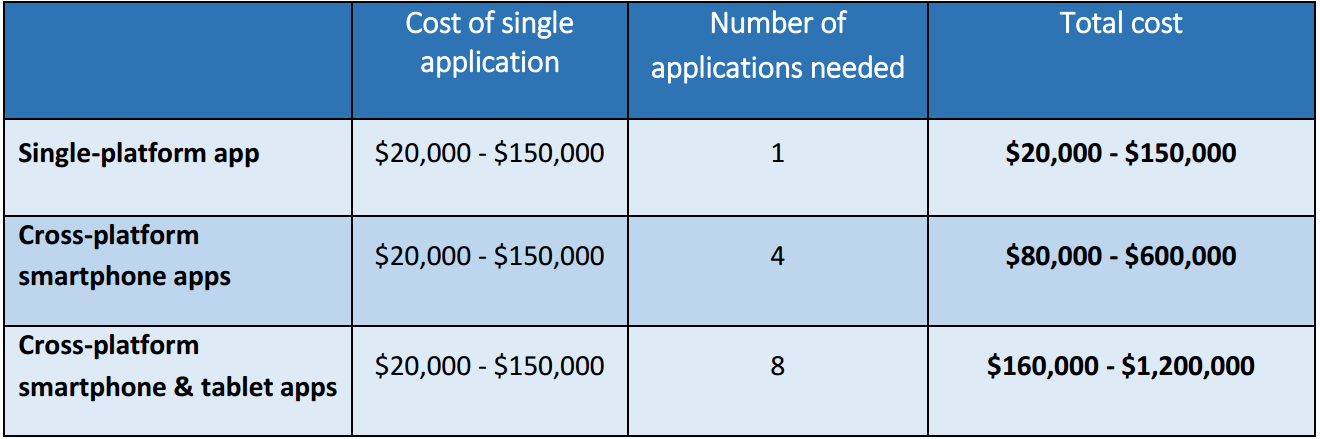
\includegraphics[width=0.8\linewidth]{./img/kostenNativeEntwick}
 \caption[Kosten: Native Entwicklung]{Kostenbeispiel der  Nativen Entwicklung \parencite[Quelle:][]{kostenNativApp}}
 \label{fig:kostenNativeEntwick}
 \end{figure}

Der Erfolg von Frameworks wie beispielsweise \nameref{subsec:phonegap} oder \nameref{subsec:titanium} basiert unter anderem darauf, dass die Entwicklung plattformunabhängig von statten geht wodurch die Entwicklungsdauer deutlich minimiert wird.
Nichts desto trotz stellen alle plattformübergreifende Frameworks eine Abstraktion zu den nativen \ac{SDK}'s da.
Dies bringt zwar auf der einen Seite eine komfortable und zügig Entwicklung mit sich, allerdings erhöht sich auf der anderen Seite auch die Abhängigkeit gegenüber dem eingesetzten Frameworks.
Solche Abhängigkeiten können sich unter anderem in der Update-Politik niederschlagen.
Vor der Auswahl des Frameworks sollte unbedingt eine Recherche über Update-Intervalle sowie die Stabilität des aktualisierten Frameworks durchgeführt werden.
Diese Punkte sollten, speziell beim erstmaligen Einsatz des Frameworks, besonders berücksichtigt werden, da sie sich deutlich auf die Qualität des Produktes auswirken können. 




\subsection*{Erweiterbarkeit der Zielplattformen}\label{sec:erweiterbarkeit-der-zielplattformen}

Der Markt für mobile Betriebssystem ist hoch dynamisch. 
In den letzten fünf Jahren wurde der Marktführer Symbian fast zur Gänze vom Markt verdrängt, während Android vom unbekannten- zum meist genutzten Betriebssystem aufgestiegen ist (siehe Abb.: \ref{fig:MarktanteilMobile} - \nameref{fig:MarktanteilMobile}). 


\begin{figure}[h]
\centering
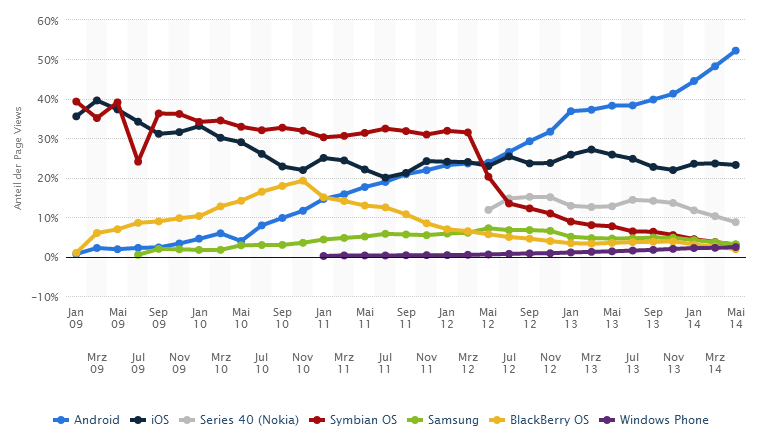
\includegraphics[width=0.9\linewidth]{./img/MarktanteilMobile}
\caption[Marktanteile der führenden mobilen Betriebssysteme]{Marktanteile der führenden mobilen Betriebssysteme an der Internetnutzung mit Mobilgeräten weltweit von Januar 2009 bis Mai 2014 \parencite[Quelle:][]{statistaMarktMobil}}
\label{fig:MarktanteilMobile}
\end{figure}

\mbox{}\\
Diese Dynamik bringt für die Applikation-Entwicklung sowohl Vor- als auch Nachteile mit sich. 
Durch den harten Wettkampf zwischen den einzelnen Plattformen sind die Hersteller darum bemüht, die bestehende Basis der Applikations-EntwicklerInnen zu halten beziehungsweise zu erweitern.
Auf der anderen Seite kann die Fluktuation der Marktanteile zu einem Risiko für die eigenen Projekt werden, wenn diese nicht in der Lage sind, sich an die aktuellen Trends anzupassen.
Der Einsatz von plattformunabhängig Frameworks in der Entwicklung kann dabei deutlich zur Flexibilitäts-Steigerungen beitragen.   
Eine Möglichkeit besteht darin, die Implementierung des Projektes auf der Basis des \nameref{subsec:phonegap} Framework's durchzuführen.
Wie die \nameref{chap:state_of_the_art}-Analyse ergeben hat, unterstützt das \nameref{subsec:phonegap}-Framework die meisten Plattformen.
Zur Erzeugung einer nativen Container-Applikation für die  unterstützte Zielplattform muss neben der PhoneGap-Infrastruktur auch das jeweilige \ac{SDK} vorhanden sein.
Neben der Unterstützung von diversen Mobilen Betriebssystemen kann \nameref{subsec:phonegap} auch Desktop-Applikationen für Microsoft Windows8 sowie Canonical Ubuntu erzeugen. \parencite[vgl.:][]{phonegapPlatformGuides}\\
\newpage
\section{Schlusswort}\label{sec:schlusswort}
Die zügigen Trend-Wechsel sowie die kurzen Entwicklungszyklen von Plattformen fordern der Planung und Entwicklung von mobilen Applikationen ein hohes Maß an Flexibilität und Umsicht ab. 
Nur durch kontinuierliche Recherchen, Fort- und Weiterbildung sowie Konsultation von Fachzeitpublikationen lässt sich der Überblick über aktuelle Trends, \ac{UI}-Designs und unterstützende Frameworks nicht verlieren.
Allerdings reicht das Wissen über die vorhandenen Technologien nicht aus. 
Wie so oft werden die Vor- und Nachteile erst durch ein gewisses Maß an Erfahrung ersichtlich.
Abschließend kann gesagt werden, dass es im Moment keine allumfassende Lösung für die Multiplattform-Entwicklung gibt.
Somit sollte die Auswahl schlussendlich auf der Basis der Prioritäten und Bedürfnissen des Projektes und dessen Infrastruktur gewählt werden.

\end{document}